\documentclass[11pt,a4paper]{article}
\usepackage[top=3cm, bottom=2cm, left=3cm, right=2cm]{geometry}
\usepackage[utf8]{inputenc}
% \usepackage[T1]{fontenc}
\usepackage{amsmath, amsfonts, amssymb}
\usepackage{siunitx}
\usepackage[brazil]{babel}
\usepackage{graphicx}
\usepackage[margin=10pt,font={small, it},labelfont=bf, textfont=it]{caption}
\usepackage[dvipsnames, svgnames]{xcolor}
\DeclareCaptionFont{MediumOrchid}{\color[svgnames]{MediumOrchid}}
\usepackage[pdftex]{hyperref}
\usepackage{natbib}
\bibliographystyle{plainnat}
\bibpunct{[}{]}{,}{s}{}{}
\usepackage{color}
\usepackage{footnote}
\usepackage{setspace}
\usepackage{booktabs}
\usepackage{multirow}
\usepackage{subfigure}
\usepackage{fancyhdr}
\usepackage{leading}
\usepackage{indentfirst}
\usepackage{wrapfig}
\usepackage{mdframed}
\usepackage{etoolbox}
\usepackage[version=4]{mhchem}
\usepackage{enumitem}
\usepackage{caption}
\DeclareCaptionLabelFormat{figuras}{\textcolor{CarnationPink}{Figura \arabic{figure}}}
\captionsetup[figure]{labelformat=figuras}

\makeatletter
\renewcommand\tagform@[1]{\maketag@@@{\color{CarnationPink}(#1)}}
\makeatother

\renewcommand{\theequation}{Eq. \arabic{equation}}
\renewcommand{\thefigure}{Fig. \arabic{figure}}

\setlist[itemize]{label=\textcolor{CarnationPink}{$\mathbf{\square}$}}

\setlist[enumerate]{label=\textcolor{CarnationPink}{\arabic*.}, align=left}


\newcounter{exemplo}

\NewDocumentEnvironment{exemplo}{ O{} }{%
\allowbreak
\setlength{\parindent}{0pt}
  \begin{mdframed}[
  leftline=true,
  topline=false,
  rightline=false,
  bottomline=false,
  linewidth=2pt,
  linecolor=CarnationPink,
  frametitlerule=false,
  frametitlefont=\Large\bfseries\color{CarnationPink},
  frametitle={\color{CarnationPink}\normalfont\bfseries #1},
  ]
}{%
  \end{mdframed}
}

\setlength{\fboxsep}{10pt}
\setlength{\fboxrule}{1pt}
\usepackage{float}
\renewcommand{\thefootnote}{\alph{footnote}}
\usepackage{url}
\hypersetup{
    colorlinks=true,
    linkcolor=cyan,
    filecolor=cyan,      
    urlcolor=cyan,
    citecolor=cyan,
    pdftitle={Resumos}
}
\pagestyle{fancy}
\fancyhf{}
\renewcommand{\headrulewidth}{0pt}
\rfoot{Página \thepage}

\title{Resumo}
\author{Tratamento com Elétrons e Braquiterapia \nocite{*}}
\date{\textit{Dalila Mendonça}}
\begin{document}
	\maketitle


\begin{exemplo}[7. Tratamento com Elétrons]
    \begin{itemize}
        \item Os elétrons perdem sua energia no meio através de interações colisionais (ou seja, ionização e excitação) e interações radiativas (bremsstrahlung). Na terapia com elétrons, as perdas radiativas só se tornam significativas em energias mais altas e materiais de alto Z.
        
        \item A figura abaixo mostra como é a PDP de um feixe de elétrons. As três principais regiões da curva são:
        
            \begin{enumerate}[label=label=\textcolor{CarnationPink}{\roman*.}]
                \item A região de buildup causada pelo espalhamento lateral dos elétrons que aumenta com o aumento da energia dos elétrons;
                \item A região da queda acentuada de dose, começando em torno da isodose de 90\%; e 
                \item A região da cauda de bremsstrahlung, onde sua magnitude aumenta com o aumento da energia.
            \end{enumerate}
        
            \begin{center}
                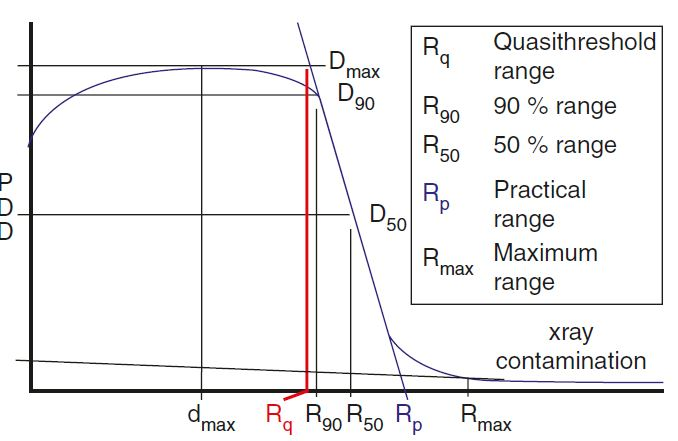
\includegraphics[width=0.5\textwidth]{Imagens/pdpEletrons.JPG}
            \end{center}

        \item O alcance prático ($R_p$) é o parâmetro que determina a profundidade de penetração do elétron. O $R_p$ é definido como o ponto com o qual a tangente da porção descendente da curva de dose na profundidade tem interseção com a curva de extrapolação da cauda de bremsstrahlung. O Alcance prático (em cm) é aproximadamente 1/2 da energia do elétron incidente (em MeV).
        
        \item Ao alterar a SSD em um feixe de elétrons, o comportamento da PDP será praticamente o mesmo, haverá um efeito mínimo na curva da PDP devido a pequena profundidade de penetração do feixe. No entanto, para altas energias de elétrons, o $R_{90}$ (profundidade distal recebendo 90\% da dose, ou seja o alcance de 90\% da dose) será deslocado distalmente alguns milímetros à medida que a SSD aumenta.
        
        \item O $R_{90}$ varia conforme o tamanho de campo. Quando o tamanho de campo está acima de um valor limite, não ocorrerá variação da dose na profundidade. Abaixo desse valor limite, que varia para cada energia de feixe, haverá uma variação significativa da dose na profundidade. Nesses casos, o $R_{90}$ é deslocado cada vez mais em direção à superfície à medida que o tamanho de campo diminui. O $R_p$, por outro lado, é dependente apenas a energia do feixe e portanto não depende do tamanho de campo se mantendo inalterado frente à mudanças do tamanho de campo.
    
        \item Diferentemente dos feixes de fótons, em que a dose na superfície diminui conforme a energia do feixe aumenta, para os feixes de elétrons o aumento da energia faz com que a dose na superfície aumente, de aproximadamente 75\% para 90\% da dose prescrita. O efeito poupador da pele é mínimo para feixes de elétrons e praticamente inexistente em feixes de elétrons de alta energia. 

        \item A colimação dos feixes de elétrons podem ser feitas diretamente na pele ou utilizando um bloco com o recorte da região de tratamento (``cutout''), acoplado ao cone de elétrons. A principal vantagem em utilizar uma colimação diretamente na pele ao invés de utilizar o bloco é que a penumbra é muito mais nítida quando comparado àos cutouts. A colimação na pele é útil para:
        
            \begin{itemize}[label=\textcolor{CarnationPink}{\textopenbullet}]
                \item Tratamentos com campos pequenos;
                \item Fornecer máxima proteção em estruturas críticas adjacentes;
                \item Reduzir a penumbra abaixo do bolus;
                \item Reduzir a penumbra abaixo de um gap de ar extendido ($>$ 5 cm);
                \item Reduzir a penumbra em terapia de elétrons com arco. 
            \end{itemize}
        
        \item A profundidade útil de um feixe de elétrons (em centímetros) é o ponto aproximado onde ocorre as linhas de isodose de 80\% a 90\%, onde $R_{80}(cm) \sim 1/3 E(MeV)$ ou $R_{90}(cm) \sim 1/3.3 E(MeV)$, no entanto $E/4$ também tem sido utilizado para aproximar o $R_{90}$. Porém é importante checar a PDP para um tamanho de campo específico para escolher a energia correta para a profundidade de tratamento necessária. 
        
        \item Existe uma contaminação de raio-x no feixe de elétrons que é resultado da interação de bremsstrahlung dentro do cabeçote do acelerador (que podem acontecer nas folhas espalhadoras, câmaras de ionização, colimadores, etc \dots) e no corpo do paciente. A Contaminação com raios-x aumenta com o aumento da energia, e os valores típicos para a contaminação são:  0.5\% até 1\% para feixes de 6 MeV até 12 MeV; 1\% até 2\% para feixes de 12 MeV até 15 MeV; e 2\% até 5\% para feixes de 15 MeV até 20 MeV.
        
        \item O Bolus é utilizado em tratamentos com eletrons para três finalidades:
        
            \begin{enumerate}[label=label=\textcolor{CarnationPink}{\roman*.}]
                \item Reduzir as irregularidades da superfície;
                \item Limitar a penetração do feixe de elétrons em certos lugares; e
                \item Aumentar a dose na superfície.
            \end{enumerate}
        O Bolus é feito de um material tecido-equivalente (Z) os materiais mais comuns de bolus são cera, gaze de parafina, superflab e outros plásticos flexíveis.

        \item Caso as PDPs para os campos quadrados $L \times L$ e $W \times W$ sejam conhecidas, a PDP para um campo retangular $L \times W$ em duma determinada profundidade d pode ser determinada a partir da PDP dos campos quadrados através da seguinte relação:
        
            $$PDP(d, L \times W) = \sqrt{PDP(d, L \times L) \cdot PDP(d, W \times W)}$$

        \item Os campos de elétrons são normalmente definidos para que sua incidência seja perpendicular à superfície do paciente. Caso a incidência seja oblíqua à superfície a PDP do feixe de elétrons será modificada, de modo que a incidência oblíqua irá acarretar em:
        
            \begin{enumerate}[label=label=\textcolor{CarnationPink}{\roman*.}]
                \item um aumento na dose na superfície;
                \item uma dose máxima mais alta;
                \item um deslocamento do $R_{90}$ em direção à superfície; 
            \end{enumerate}

        Estas mudanças são mais significantes em ângulos de obliquidade $>$ \ang{30}.

        \item Ao tratar uma região contendo uma cavidade de ar, a dose na região distal da cavidade nasal é aumentada devido ao maior espalhamento que ocorre em direção a cavidade de ar, enquanto que a dose lateral e distal à  cavidade de ar diminui (ambos os efeitos são devido à perca de equilíbrio lateral). Além disso, o alcance dos elétrons aumenta devido à baixa atenuação nessa região. Portanto, ao tratar regiões que atravessam as cavidades nasais, por exemplo tratamentos de septo nasal, devem ser utilizados tampões nasais para substituir a perda do meio espalhador.
        
        \item Ao tratar uma região que irá atravessar um tecido ósseo, a dose diretamente distal ao osso é diminuída enquanto a dose lateral e distal ao osso é aumentada. Ambos destes efeitos ocorrem devido à perda de equilíbrio de espalhamento lateral. Com o osso, haverá mais espalhamento saindo do osso do que entrando nele o que é oposto ao que ocorre quando o feixe atravessa uma cavidade de ar. 
            
        \item Nos casos de superfícies irregulares com heterogeneidades internas, levarão a uma distribuição de dose complexa com pontos quentes e frios na região de tratamento. Normalmente, para uma protuberância, como o nariz, os pontos quentes estarão em ambos os lados da protuberância e um ponto frio atrás dela; Enquanto que para uma cavidade, como perto do meato acústico externo, a base da cavidade estará quente enquanto seus lados estarão frios. Nesses casos, a utilização de bolus poderá ajudar a aliviar esses efeitos. 
        
        \item Ao utilizar um bolus em um tratamento de elétrons, de forma que o bolus cubra apenas uma parte do campo de tratamento, a borda do bolus irá atuar semelhante a uma protuberância, causando um ponto quente fora do bolus e um ponto frio dentro do bolus. Este efeito pode ser evitado afunilando a borda do bolus. 
        
        \item Ao desenvolver colimações internas para feixes de elétrons, como aquelas utilizadas em Radioterapia Intra-Operatória (IORT) feitas em chumbo, deve-se atentar às seguintes considerações:
        
            \begin{enumerate}[label=label=\textcolor{CarnationPink}{\roman*.}]
                \item A espessura do colimador deve ser suficiente para parar a radiação; e
                \item O retroespalhamento do elétron pode ser significativo e deve ser considerado no desenvolvimento da colimação, revestindo o colimador com plástico, cera ou cerâmica para blindar os elétrons retroespalhados na blindagem que podem contribuir para um aumento indesejado da dose na região de tratamento. 
            \end{enumerate}

        \item Ao utilizar campos de elétrons adjacentes, forma da isodose na profundidade para os feixes de elétrons levará a formação de pontos quentes e frios na profundidade da adjacência dos campos. Essa heterogeneidade da dose pose ser reduzida, deslocando a borda do feixe em $\pm 1$ cm ao longo do tratamento. 
        
        \item Na IORT, não é possível realizar uma tomografia de planejamento pois o tratamento ocorre no momento da cirurgia. Portanto, o cálculo das MUs necessárias para entrega da dose é feito manualmente, com base em uma profundidade estimada ou determinada no momento da cirurgia, utilizando campos moldados com chumbo ou utilizando aplicadores específicos para a técnica. 
        
        \item Na Terapia em Arco de Elétrons, o gap de ar entre o colimador secundário e o paciente normalmente é maior que o normal, o que irá causar uma maior penumbra. Este efeito pode ser corrigido utilizando uma colimação na pele para deixar a penumbra mais nítida e girar o arco aproximadamente \ang{15} além da borda da área de tratamento.
        
        \item Ao definir a forma da abertura do bloco para tratamento de elétrons, uma possibilidade é desenhar o formato da região de tratamento em um molde em contato com a superfície do paciente. Estima-se que há uma margem de aproximadamente 1 cm entre a borda do alvo e a borda do recorte no bloco quando ambos estão projetados no isocentro. (testar isso aqui!!!)

        \item Conforme a energia do feixe de elétrons aumenta a dose na superfície, a profundidade da isodose de 90\%, o alcance prático e a contaminação com bremsstrahlung também aumenta. A profundidade de dose máxima varia irregularmente com a energia e com o modelo do acelerador.
        
        \item As curvas de isodose de para os feixes de elétrons devem ser determinadas especificamente para cada máquina para as mesmas energias e tamanhos de campo em comum com outras máquinas (não pode-se utilizar os "golden data" para alimentar as pastas de cálculo). Isto se deve ao espalhamento dos elétrons por diferentes componentes físicos presentes no caminho do feixe, que pode mudar de um acelerador para o outro, gerando uma distribuição de dose diferente entre aceleradores apesar de manter as mesmas condições de medida.
        
        \item O retroespalhamento dos elétrons aumenta com o aumento do número atômico e diminui com o aumento da energia do elétron. 
        
        \item Para determinar a dose em um ponto utilizando terapia em arco de elétrons, pode-se medir a dose nesse ponto em um phantom cilíndrico, ou integrar a distribuição de isodose no ponto.
        
        \item Ao utilizar blindagens de feixes de elétrons, diretamente em contato com o pacientes, a dose no tecido em contato com a blindagem irá aumentar pois a blindagem causa o retroespalhamento dos elétrons. Portanto é importante cobrir a proteção com um filtro de número atômico inferior ao da proteção, por exemplo utilizar cera ou plástico nas proteções oculares. É importante lembrar que, o retroespalhamento sempre causará maior dose na região adjacente do material de menor número atômico.
        
        \item A densidade eletrônica relativa de um meio  é determinada em relação a densidade eletrônica da água (meio com o qual o feixe é caracterizado). Por exemplo, a densidade eletrônica relativa para o osso compacto é de 1.6, para o osso esponjoso é de 1.1 e para o pulmão é de 0.2, comparados à densidade eletrônica da agua.

        \item Para determinar a espessura de chumbo necessária para a confecção de um bloco de chumbo utiliza-se a estimativa $T(chumbo)(mm) = 0.5\;mm/MeV$, podendo ser adicionado 1 mm como uma medida de segurança. Normalmente são utilizados blocos feitos de Cerrobend que é aproximadamente 20\% menos denso que o chumbo e portanto, a espessura utilizando o Cerrobend é de 1.2 x T(chumbo). 

        
        \item Diferentemente de um feixe de fótons, que parecem ser originados a partir de um ponto focal (fonte) localizado no alvo de raios-x onde foram produzidos, o feixe de elétrons apresenta um comportamento diferente, de modo que o feixe parece se originar em um ponto virtual no espaço (e não a partir da folha espalhadora), e a posição deste ponto pode mudar dependendo da energia do feixe e do tamanho de campo. Diversas medidas são realizadas à diferentes distâncias que são plotadas em um gráfico para determinar através da extrapolação da curva a posição virtual da fonte, no qual normalmente está logo acima da folha espalhadora. 
        
        \item A posição virtual da fonte é utilizada para calcular a distância da fonte virtual até a superfície ($SSD_{eff}$) afim de estimar o output do feixe com base no inverso quadrado da distância em tratamentos com a SSD estendida. 
        
        \item O feixe estreito de elétrons que sai da guia aceleradora é praticamente monoenergético. No entanto, até chegar ao paciente, o feixe irá interagir com as folhas espalhadoras, colimadores, ar e outras estrutura que estão no seu caminho. Estas interações resultam em uma alargamento do espectro de energia do feixe de modo que a energia média na superfície do paciente é menor que a energia do feixe inicial criado na gia aceleradora.
        
        \item As linhas de alta isodose e baixa isodose se comportam de forma diferente em relação ao tamanho de campo na superfície. As linhas de alta isodose (90\%) são mais estreitas de modo que cobre uma região menor em relação ao tamanho de campo na superfície enquanto que as linhas de baixa isodose são mais largas de modo que cobrem uma região mais larga que o tamanho de campo na superfície. Observando pelo BEV, a isodose de 90\% estaria para dentro da borda do campo e a isodose de 20\% estaria para fora da borda do campo. 
        
        \item Os feixes elétrons são frequentemente utilizados para tratar tumores de pele superficiais, tumores em pequenas profundidades, leitos tumorais e cicatrizes queloidianas. No tratamento de mama, os elétrons podem ser utilizados para tratar a mamária interna, a parede do tórax após a mastectomia (plastrão) e boost (reforço) em leitos tumorais.
        

        \item Ao utilizar um bolus no tratamento com elétrons, o bolus deve ser colocado em contato direto com a  superfície da pele evitando a presença de gaps de ar entre o bolus e pele. A existência de gaps de ar entre o bolus e a pele além de promover um aumento na penumbra do feixe faz com que a dose superficial seja menor que a dose esperada. Isto ocorre devido aos elétrons que são espalhados pelo bolus conseguirem viajar para fora do campo na região do gap de ar, diminuindo a fluência de elétrons que incidem na pele.

    \end{itemize}
\end{exemplo}

\begin{exemplo}[8. Braquiterapia]
    \textcolor{CarnationPink}{Braquiterapia}
    \begin{itemize}
        \item A Braquiterapia é um procedimento especial da Radioterapia que utiliza fontes radioativas colocadas a curtas distâncias do alvo de tratamento. A Braquiterapia fornece distribuições de dose com alto índice de conformidade dentro do volume alvo devido as sementes radioativas (ou fontes) serem colocadas diretamente dentro do alvo ou em suas proximidades.
        
        \item Os tipos de Braquiterapia são:
        
            \begin{itemize}[label=\textcolor{CarnationPink}{\textopenbullet}]
                \item \textcolor{CarnationPink}{\textbf{Braquiterapia Intersticial:}} As fontes radioativas são colocadas diretamente no tecido alvo, ou temporariamente ou permanentemente;
                \item \textcolor{CarnationPink}{\textbf{Braquiterapia Intracavitária:}} As fontes radioativas estão contidas dentro de um aplicador inserido nas cavidades do corpo, como a vagina ou o útero;
                \item \textcolor{CarnationPink}{\textbf{Braquiterapia Intraluminal:}} Se trata de uma subclasse da Braquiterapia Intracavitária, no qual as fontes radioativas são inseridas no lúmen do paciente como os vasos sanguíneos, brônquio, esôfago ou ducto biliar; (\textit{Lúmen é um espaço interno ou cavidade dentro de uma estrutura com formato de tubo num corpo, como as artérias e o intestino})
                \item \textcolor{CarnationPink}{\textbf{Braquiterapia Superficial:}} As fontes radioativas sao colocadas em placas superficiais o moldes que são então colocados na área de tratamento como o olho ou a pele. 
            \end{itemize}

        \item Os sistemas de carregamento das fontes em Braquiterapia são:
        
            \begin{itemize}[label=\textcolor{CarnationPink}{\textopenbullet}]
                \item \textcolor{CarnationPink}{\textbf{Pré-Carregamento Manual:}} Utilizado para sementes de baixa taxa de dose como as utilizadas para tratamento de próstata ou placas oftalmológicas;
                \item \textcolor{CarnationPink}{\textbf{Pós-Carregamento Manual:}}  Atualmente esta técnica não é utilizada com frequência;
                \item \textcolor{CarnationPink}{\textbf{Pós-Carregamento Remoto:}} Técnica utilizada para Braquiterapia de Alta taxa de dose;
            \end{itemize}

        \item O tempo de duração do implante é classificado como:
        
            \begin{itemize}[label=\textcolor{CarnationPink}{\textopenbullet}]
                \item \textcolor{CarnationPink}{\textbf{Implante Permanente:}} As fontes radioativas são permanentemente implantadas dentro do tumor;
                \item \textcolor{CarnationPink}{\textbf{Implante Temporário:}} As fdntes radioativas são implantadas dentro ou perto do tumor e então são removidas uma vez que a dose de radiação prescrita para aquela fração tenha sido entregue.
            \end{itemize}

        \item O ICRU 38 Classifica as faixas de taxa de dose da seguinte forma:
        
            \begin{itemize}[label=\textcolor{CarnationPink}{\textopenbullet}]
                \item \textcolor{CarnationPink}{\textbf{Baixa Taxa de Dose (LDR):}} 0.4 Gy/h - 2.0 Gy/h. Utilizada para implantes permanentes ou pós-carregadores manuais. 
                \item \textcolor{CarnationPink}{\textbf{Média Taxa de Dose (MDR):}} 2Gy/h - 12Gy/h. Pós-carregadores de braquiterapia de taxa de dose pulsada (PDR) foram desenvolvidos neste intervalo de taxa de dose para replicar os efeitos radiobiológicos de um tratamento de LDR em termos da duração total do tratamento, porém emitindo pulsos de radiação com duração variando entre 5 min até 10 min por hora, e não durante todo o tempo de tratamento como ocorre na LDR.
                \item \textcolor{CarnationPink}{\textbf{Alta Taxa de Dose (HDR):}} $>$ 12 Gy/h. A Braquiterapia HDR utiliza uma fonte com alta atividade, normalmente uma fonte de \ce{^{192}Ir} com 10 Ci. O tratamento é entregue utilizando técnicas controladas remotamente. A taxa de dose típica em um tratamento com HDR varia em torno de 100 Gy/h até 300 Gy/h.
            \end{itemize}

        \item Os radionuclídeos mais utilizados em braquiterapia são:
        
            \begin{itemize}[label=\textcolor{CarnationPink}{\textopenbullet}]
                \item Radiação gama de alta energia, como por exemplo: Cs-137, Ir-192 e Co-60;
                \item Radiação gama de baixa energia, como por exemplo: Ir-125 e Pd-103;
                \item Radiação Beta, como por exemplo: P-32, Ru-106, Sr-90 e Y-90;
            \end{itemize}

            Portanto radiação gama e beta são os tipos de radiação mais utilizados em braquiterapia. Muito raramente são utilizados nêutrons (Cf-252) e partículas alfa. 


        \item A intensidade da fonte (força da fonte) pode ser especificada em termos da intensidade do Kerma no ar (força Kerma ar - U) para emissores gama; e pode ser especificada em termos de Becquerel (Atividade) (MBq ou GBq) para emissores beta. As unidades Ci e mCi são unidades antigas mas ainda são comumente utilizadas para emissores gama.
        
        \item Os radionuclídeos utilizados em braquiterapia podem estar no estado sólido, líquido e gasoso (como ocorre em fontes de Xe-133). Fontes sólidas são seladas através do encapsulamento em uma camada de metal.
        
        \item As principais vantagens em tratamentos HDR quando comparado a tratamentos LDR são que: $(i)$ O tratamento HDR requer um procedimento ambulatorial, não sendo necessária a internação do paciente; $(ii)$ é um tratamento que requer o uso de afterloaders remotos, levando a uma redução ou eliminação da exposição de radiação da equipe envolvida no processo; $(iii)$ Permite maior controle da distribuição de dose pois a movimentação da fonte permite a otimização da distribuição de dose ajustando o tempo de parada em cada posição de parada para cada canal do afterloader, podendo ser catéter ou agulhas; $(iv)$ É um tratamento com maior estabilidade no posicionamento do aplicador pois leva menos tempo para entregar a dose (menos de uma hora)minimizando a movimentação dos aplicadores durante o tratamento;  $(v)$ A duração mais curta de tratamento permite que seja feito um deslocamento físico de estruturas sadias durante o tratamento, diminuindo a dose recebida no tecido normal; e $(vi)$ devido ao pequeno tamanho das fontes de HDR é possível utilizar aplicadores menores se adequando melhor à estruturas que necessitam de uma cobertura em uma área ou região pequena/estreita.
        

        \item As principais desvantagens em tratamentos HDR quando comparado a tratamentos LDR são que: $(i)$ Um tratamento HDR requer um alto investimento uma vez que os afterloaders possuem alto custo; $(ii)$ Os efeitos radiobiológicos da HDR causam uma maior toxicidade no tecido normal pois a medida que a taxa de dose aumenta, a radiossensibilidade, ou seja, o dano por unidade de dose, aumenta tanto para o tecido tumoral quanto para o tecido normal, porém a radiossensibilidade do tecido normal aumenta mais rapidamente do que a radiossensibilidade do tecido tumoral, aumentando a probabilidade de causar danos ao paciente ao mesmo tempo que o tumor é tratado. Para justificar sua utilização faz-se uso das vantagens de otimização, geometria, estabilidade e redução de dose em tecidos normal além de um esquema de tratamento com múltiplas frações; e $(iii)$ caso o equipamento apresente um mau funcionamento, ou se um paciente estiver em uma situação de emergência, o risco de exposição acidental à radiação é muito maior tanto para o paciente quanto para a equipe no tratamento HDR.
        
        \item Os recursos de segurança e os intertravamentos (interlocks) operacionais necessários para um afterloader HDR são: $(i)$ Sistema Audiovisual; $(ii)$ Monitores de radiação e indicadores de tratamento (luz vermelha indicando que a fonte está exposta); $(iii)$ Interlock de porta;  $(iv)$ Botões de emergência; $(v)$ Manivela de emergência; e $(iv)$ Bateria Reserva (nobreak).
        
        \item O método atual para calcular a taxa de dose no tecido para uma fonte radioativa é através do formalismo modular descrito no TG-43 que determina a taxa de dose em um meio homogêneo de água, não considerando a heterogeneidade do tecido.
        
        \item A anisotropia se refere a dependência direcional da fluência para uma fonte devido à localização do material radioativo dentro da fonte e devido as diferenças na construção das fontes e nas espessuras das paredes do encapsulamento.
        
        \item Para distâncias maiores que poucos mm o principal fator para determinar a taxa de dose da fonte é o fator do inverso quadrado da distância.
        
        \item Para localizar uma fonte de radiação perdida, o detector que deve ser utilizado é p Geiger Muller; Porém, para avaliar um paciente antes de ele ter alta, o instrumento indicado é a câmara de ionização (que irá indicar diretamente a taxa de dose). A câmara de ionização utilizada nessa avaliação deve conter um grande volume sensível com ar pressurizado.
        
        \item As novas fontes devem ser calibradas antes de serem utilizadas nos tratamentos dos pacientes utilizando um sistema de dosimetria com calibração rastreável pelo Laboratório Padrão Secundário (que é rastreável pelo laboratório padrão primário Instituto Nacional de Padrões e Tecnologias NIST). O sistema de dosimetria consiste tipicamente em uma câmara poço e um eletrômetro capaz de fazer a leitura em modo corrente. Para a atividade da fonte na faixa de mCi, as leituras de corrente pelo eletrômetro são da ordem de \qty{e{-11}}{A}. Para uma fonte de HDR, cuja atividade é em torno de 10 Ci, a corrente medida pelo eletrômetro é da ordem de \qty{e{-7}}{A}. A corrente medida pode então ser convertida em atividade da fonte.
        
        \item Ao realizar uma calibração na fonte, algumas correções devem ser feitas na leitura fornecida pelo eletrômetro. Se a câmara posso for aberta para a atmosfera, que acontece para a maioria, é necessário aplicar as correções de temperatura e pressão. Além disso, pode ser necessário aplicar uma correção para escala de leitura do eletrômetro. 
        
        \item A NCR (Comissão Reguladora Nuclear) exige que uma pessoa/instituição licenciada mantenha um registro de inventário para todos materiais radioativos. O registro deve conter o tipo de fonte (isótopo), intensidade da fonte e sua localização. As fontes permanentemente implantadas em um paciente não estão sujeitas a esse controle de inventário uma vez que o paciente tenha sido liberado da instalação. 

    \end{itemize}

    \textcolor{CarnationPink}{Braquiterapia LDR}
    \begin{itemize}
        \item Os principais isótopos utilizados em implantes permanentes são o Iodo-125, o Paládio-103 e o Césio-131.  Eles são utilizados devido emitirem fótons com uma energia média baixa, sendo \ce{^{125}I} = \qty{0.028}{MeV}, \ce{^{103}}Pd = \qty{0,021}{MeV} e \ce{^{131}Cs} = \qty{0,029}{MeV}, e por terem um tempo de meia vida relativamente curto, sendo \ce{^{125}I} = \qty{59.4}{dias}, \ce{^{103}Pd} = \qty{17}{dias} e \ce{^{131}Cs} = \qty{9.7}{dias}. Portanto, devido a baixa energia dos fótons emitidos, essas fontes irão tratar apenas o tumor devido ao acentuado falloff de dose alcançado para fótons de baixa energia.
        
        \item No implante de próstata existem alguns parâmetros dosimétricos que devem ser considerados. Para implantes permanentes utilizando \ce{^{125}I}, é prescrita uma dose total de 144 Gy para cobrir toda a próstata delineada na imagem de ultrassom, para o \ce{^{103}}Pd é prescrita a dose de 125 Gy e para o \ce{^{131}Cs} é prescrita a dose de 115 Gy.
            \begin{enumerate}[label=label=\textcolor{CarnationPink}{\alph*)}]
                \item  O volume de próstata (CTV) recebendo 150\% da dose de prescrição ($V_{150\%}$) deve ser $\leq 50\%$, variando normalmente entre 40\% e 50\%.
                \item O volume do CTV recebendo 200\% da dose de prescrição deve ser $\leq 20\%$, variando normalmente entre 10\% e 20\%.
                \item O volume de CTV que recebe 100\% da dose prescrita deve ser de no mínimo 95\%, ou seja, $V_{100\%} \geq 95\%$.
                \item A dose que cobre 90\% do volume do CTV deve ser maior que a dose de prescrição, ou seja, $D_{90\%} > 100\%$. 
            \end{enumerate}

        \item Para implantes de próstata, pode-se realizar uma aproximação quanto à anisotropia, de modo que seja determinada apenas em função da distância sem informação direcional em função da orientação da semente dentro do implante.
        
        \item A NCR estabelece um critério de liberação para pacientes com implantes permanentes de próstata. A NCR estabelece que uma pessoa licenciada pode autorizar a liberação de seu controle, qualquer indivíduo que tenha recebido um material radioativo não selado ou implantes contendo material radioativo caso o equivalente de dose efetiva total em qualquer outro indivíduo devido a exposição ao indivíduo liberado não exceda 5 mSv (0.5 rem). Em implantes de próstata, esta condição é satisfeita se a taxa de exposição medida a 1m do paciente é $<$ 1mR/h.

        \item Após a implantação das sementes, é realizada uma dosimetria pós implante através de uma imagem de tomografia realizada aproximadamente 30 dias depois do implante das sementes de braquiterapia de próstata. Este tempo é necessário para que o inchaço da glândula devido à edemas tenha diminuído. A Dosimetria pós implante é realizada principalmente como uma medida de garantia da qualidade para o procedimento de implante e também tem sido utilizada para fins regulatórios (isto é, para definir um ``evento médico'').
        
        \item Em um procedimento de implante de próstata, o paciente é colocado em posição de litotomia dorsal (posição onde o corpo está deitado com a face voltada para cima, mas com os pés elevados e com uma flexão de 90 graus do quadril e joelho) sob anestesia geral. As fontes radioativas são implantadas através do períneo utilizando agulhas pré-carregadas contendo sementes soltas ou sementes dispostas em um fio. As sementes radioativas são espaçadas em pelo menos 1 cm na agulha e o número de agulhas necessárias dependerá do volume da próstata. As agulhas são normalmente dispostas para fornecer um carregamento periférico modificado de modo que menos fontes sejam posicionadas no centro da próstata perto da uretra. As agulhas são inseridas através de um template especial que é anexado a uma sonda de ultrassom transretal. As sementes também podem ser implantadas utilizando um aplicador Mick.
        
        \item Tratamentos de Melanoma Uveal e Retinoblastoma podem ser tratados com braquiterapia, utilizando uma placa superficial contendo material radioativo. As principais fontes utilizadas na braquiterapia ocular são (Iodo-I25, Rutênio-106, Paládio-103 e Césio-131). Os melanomas são tratados com uma dose de prescrição de 85 Gy em 3 ou 4 frações e os Retinoblastomas são tratados com uma dose se prescrição variando entre 40 Gy a 45 Gy entregues em duas frações. As placas oftalmológicas também protegem a cavidade ocular da radiação. 
        
        \item As placas COMS, utilizadas na braquiterapia ocular, consistem em uma blindagem de ouro com um portador silástico (borracha de silicone) contendo as sementes de Iodo-125, bem como as placas de ouro Eye Physics com sementes incorporadas. Existem placas COMS disponíveis com um encaixe para facilitar a colocação próxima ao nervo óptico. 
        
        \item A dose COMS é de 85 Gy prescrita na profundidade de no mínimo 5 mm ou no ápice do tumor, caso for maior que 5 mm. Os tempos de tratamento são normalmente em torno de 100 horas. Para COMS, a dose foi calculada usando um modelo pontual para a semente e sem considerar correções de anisotropia ou heterogeneidade. As recomendações atuais da AAPM (Associação Americana de Físicos em Medicina) são para usar uma aproximação de fonte linear e calcular para meios homogêneos de água. Incluídos no relatório do TG 129, estão os dados para correções de heterogeneidade. Um software como o Plaque Simulator modifica o cálculo levando em consideração a atenuação do portador silástico e as mudanças no espalhamento devido à blindagem de ouro.
        
        \item Quanto aos ensaios da atividade das sementes, a NCR exige um ensaio independente de 10\% para confirmar a precisão da atividade da semente especificada. O ensaio pode ser feito por terceiros mas a AAPM recomenda que seja feita uma checagem na instituição local.
        
        \item Quanto a proteção radiológica nos casos de pacientes submetidos à braquiterapia ocular, é necessário que os pacientes permaneçam no hospital durante o tratamento. A sala onde eles serão alojados deverá conter uma placa afixada fora da sala indicando a presença de radiação; Os pacientes devem utilizar óculos especiais com chumbo quando os visitantes ou a equipe de enfermagem estiver presente, para reduzir os níveis de exposição por um fator de 5 a 6. É necessário realizar um treinamento anual para a equipe de enfermagem com respeito à proteção radiológica. Após a alta do paciente, a sala deve ser avaliada quanto ao material radioativo. 
        
        \item Quanto a proteção radiológica nos casos de pacientes submetidos à implantes de próstata, após o procedimento de implante na sala de cirurgia, o paciente é levado para uma área de recuperação, onde será fornecido um mictório para seu uso. Após a alta, que geralmente ocorre após algumas horas, o mictório e a roupa de cama são analisados com respeito à radiação. Se alguma fonte for encontrada, ela deverá ser armazenada em um armário trancado até sua posterior remoção pela instituição responsável. Os pacientes com implantes permanentes deverão receber um cartão indicando a data e a natureza do implante, contendo informações com respeito ao isótopo e sua atividade total, juntamente com um documento informando as precauções que devem ser tomadas para minimizar a exposição a outras pessoas.
        
        \item O sistema Patterson-Parker (Manchester) foi historicamente aplicado em implantes intersticiais. O principal objetivo desse sistema é entregar uma dose uniforme em um plano ou em um volume formado por planos paralelos, a uma distância de 0.5 cm do(s) plano(s) implantado(s) dentro de $\pm$ 10\% da dose prescrita. Para alcançar esse objetivo, o sistema utiliza regras especificas para a distribuição das fontes de radiação e atividades destas fontes. Para um implante planar, quanto menor a área tratada, maior a fração da quantidade de rádio (ou radio equivalente) que deve ser colocada na periferia. O volume do implante é determinado e as tabelas são utilizadas para determinar os miligramnas-hora de Rádio por 1000 roentgens. 
        
        \item O sistema Quimby também foi historicamente aplicado para implantes intersticiais e seu objetivo é calcular a dose máxima do centro do plano de tratamento em uma distância de até 3 cm. Esse sistema depende de uma distribuição uniforme das fontes com mesma atividade. A principal diferença com o Patterson-Parker é que o sistema Patterson-Parquer utiliza uma distribuição não uniforme das fontes e pode empregar fontes com atividades variadas para alcançar uma dose uniforme no plano implantado.
        
        \item O Sistema Paris prescreve a dose em uma isodose superficial (isodose de referência). Semelhantemente ao sistema Quimby, são utilizadas fontes uniformes porém colocadas em linhas paralelas.
        
        \item Tanto o sistema Manchester Quanto o Sistema Quimby foram projetados para implantes de Rádio. Isótopos Rádio-equivalentes como o Irídio-192 e o Césio-137 podem ser calculados para esses sistemas, porém esses sistemas não são compatíveis para fontes de braquiterapia de baixa energia como as fontes de Iodo-125.
        
        \item No planejamento moderno de braquiterapia Intersticial, os sistemas como o  Manchester, Quimby e Paris foram amplamente substituídos por cálculos de dose computadorizados que entregam a soma das doses para cada ponto devido a contribuição de todas as fontes, além do uso de sistemas afterloading que permitem a avaliação prévia do plano com fontes dummy (fictícias) inseridas nas posições pré-configuradas seguido da colocação das fontes ativas após a avaliação do plano. 

    \end{itemize}

    \textcolor{CarnationPink}{Braquiterapia HDR}
    \begin{itemize}
        \item A principal fonte utilizada na Braquiterapia HDR é o Irídio-192. A meia vida do \ce{^{192}Ir} é de 74.4 dias e a energia média dos fótons emitidos é de 380 KeV. Uma fonte típica possui um diâmetro variando entre 0.3 mm até 0.6 mm e um comprimento variando entre 3.5 mm até 10 mm com uma atividade inicial de \qty{\sim 10}{Ci}.
        
        \item A NCR estabelece um limite para fuga em HDR, de modo que a radiação de fuga não possa exceder 1 mR/h a uma distância de 10 cm a partir da superfície acessível mais próxima do cofre quando a fonte estiver na posição blindada. 
        
        \item Segundo a NCR, os seguintes passos devem ser realizados antes de iniciar um procedimento HDR:
        
            \begin{enumerate}[label=\textcolor{CarnationPink}{\roman*.}]
                \item Um médico autorizado deve assinar a indicação e a prescrição escrita;
                \item O paciente deve ser identificado e verificado por dois métdos (nome e nome da mãe, data de nascimento...);
                \item O plano de tratamento deve ser checado por um físico médico;
                \item As verificações de segurança da unidade HDR pré-tratamento devem ser concluídas;
                \item Antes da entrega do tratamento, um usuário autorizado deverá verificar os detalhes do paciente e do tratamento;
                \item O tratamento deve ser supervisionado do início ao fim por um usuário autorizado e os registros de tratamento devem ser registrados.
                \item Uma monitoração de radiação pós entrega deve ser concluída;
                \item Eventos médicos devem ser registrados e reportados;
                \item Revisões periódicas pelo menos anualmente devem ser realizadas onde a fonte e a calibração devem ser testadas e registadas. 
            \end{enumerate}

        \item O \ce{^{137}Cs} é um isótopo possível para ser utilizado em braquiterapia HDR. o \ce{^{137}Cs} tém uma energia média maior que a do \ce{^{192}Ir} o que poderia ser uma vantagem pois fornece uma maior percentagens de dose na profundidade, porém energias mais altas requerem maiores requisitos de blindagem. O \ce{^{137}Cs} possui uma meia vida longa, o que demandaria uma menor frequência de troca de fonte comparado ao \ce{^{192}Ir}, no entanto o \ce{^{137}Cs} tem uma menor atividade específica o que implicaria em uma fonte maior e portanto catéteres mais largos. 

        \item Pacientes com câncer endometrial normalmente se beneficiam de braquiterapia HDR pois embora a maior marte das pacientes são submetidas a histerectomias curativas, sem um tratamento posterior, aproximadamente 12\% destas pacientes provavelmente terão uma recorrência local. Já as pacientes que receberam o tratamento profilático de cúpula vaginal tem a chance de recorrência muito reduzida.
        
        \item Para tratamentos de câncer endometrial com braquiterapia, são utilizados os cilindros vaginais como aplicadores. Os cilindros são projetados com uma variedade de diâmetros, variando entre 2 cm até 4cm, e comprimentos para melhor de conformar a anatomia da paciente. O cilindro deve ajustar-se perfeitamente à face superior da cúpula e estar em contato com as superfícies laterais da vagina. Deve-se utilizar o maior diâmetro possível do cilindro que se adeque a paciente pois quanto maior o diâmetro do cilindro mais uniforme será a distribuição de dose no alvo.
        
        \item No tratamento do ca endometrial, o alvo é definido para abranger toda a cúpula vaginal. A maior parte das pacientes tem a metade superior da vagina tratada. Dependendo da extensão da invasão do miométrio, o tratamento de radioterapia pode incluir um tratamento com radioterapia externa e um boost com braquiterapia que é sempre considerado caso tenha uma invasão superior a 50\%. Caso contrario, onde a invasão é inferior a 50\%, pode-se realizar a braquiterapia exclusiva.
        
        \item Para os casos de câncer endometrial utilizando braquiterapia HDR, normalmente é adotado um regime de 3 frações entregando 7 Gy por fração (totalizando 21 Gy) na profundidade de 0.5 cm. Porém  a dose para a braquiterapia pode variar, inclusive quando combinada com a teleterapia.
        
        \item Os principais órgãos de risco avaliados no tratamento HDR de câncer cervical são a bexiga, o reto e o sigmoide.
        
        \item No tratamento combinado de teleterapia e braquiterapia, em dose equivalente de 2 Gy por fração (EQD2), a cobertura alvo D90 deve ser igual a 100\% da prescrição. Os limites de D2cc para o sigmoide $<$75 Gy; D2cc para o reto $<$ 75 Gy e D2cc para a bexiga $<$ 95 Gy devem ser alcançados.
        
        \item o uso de um cilindro multicanais pode auxiliar a reduzir a dose na bexiga e no reto. Enquanto um cilindro vaginal padrão possui apenas o canal central por onde a fonte irá passar, o cilindro multicanais possui um canal central e entre 6 e 8 canais periféricos distribuídos ao longo da superfície do cilindro. O cilindro multicanais aumenta o controle dosimétrico através de um carregamento diferencial dos canais, o que torna possível alcançar uma distribuição de dose que reduz a dose no reto e na bexiga ao mesmo tempo que mantém a cobertura adequada do alvo. Com O cilindro padrão é possível alcançar apenas uma distribuição de dose circular, de modo que não é possível diminuir a dose nos OAR's sem comprometer a cobertura do alvo. Uma outra variação deste aplicador  é o cilindro blindado, que permite a inserção de blindagens em qualquer um dos quatro quadrantes do cilindro para reduzir a dose naquele quadrante.
        
        \item A técnica de braquiterapia 2D utiliza duas radiografias convencionais, uma anterior e outra lateral, enquanto que na braquiterapia 3D podem ser utilizadas imagens de tomografia computadorizada ou ressonância magnética. A maior vantagem em utilizar imagens volumétricas é que ao utilizar uma radiografia, embora a localização e a reconstrução da posição das fontes utilizando marcadores radiográficos sejam feitas de forma simples e precisa, não é possível visualizar tecidos moles como o tumor, o reto e a bexiga. Já em imagens volumétricas, é possível visualizar os tecidos moles e fornecer uma caracterização tridimensional da dose com respeito a cobertura do alvo e às normais.
        
        \item De acordo com o ICRU, para especificar a dose na bexiga e no reto, devem ser determinados pontos de cálculo. Para fornecer um ponto de cálculo para a bexiga, um balão de Foley é colocado na bexiga e preenchido com cerca de \qty{7}{cm^3} de contraste, e então o ponto de bexiga é definido na parte centro-posterior do balão. Já o ponto de reto é definido 0.5 cm além da parede posterior da vagina.
        
        \item A otimização no tratamento com cilindro vaginal ajusta os tempos de parada para cada posição de parada individualmente de modo que a distribuição de dose resultante fique em melhor conformidade com o volume alvo. A figura abaixo mostra a distribuição de dose para um plano sem otimização (imagem da esquerda) e um plano com otimização (imagem da direita). Os pontos de otimização, um para cada posição de parada da fonte, são normalmente colocados a uma distância de 0.5 cm da superfície lateral da vagina, ou seja, a 0.5 cm de distância da superfície do cilindro, e pontos adicionais de otimização também podem ser colocados no ápice vaginal. Sem a otimização  a distribuição de dose é oval, ficando mais quente no centro do comprimento do cilindro. A otimização reduz os tempos de parada da fonte no seu centro e aumenta o tempo de parada nas extremidades do cilindro, produzindo então uma distribuição de dose mais retangular. A figura abaixo também mostra as posições de parada da fonte (representadas por pontos no centro do cilindro), os pontos de dose utilizados para normalização e otimização (representados por cruzes), e o volume alvo clínico (representado pela linha tracejada).

            \begin{center}
                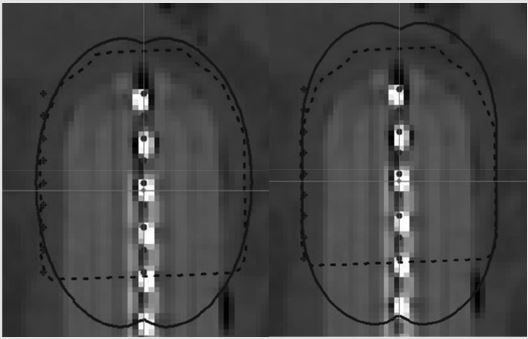
\includegraphics[width=0.5\textwidth]{Imagens/cilindroDose.JPG}
            \end{center}
            
        \item É possível utilizar braquiterapia Intersticial em pacientes ginecológicas em casos de câncer endometrial ou câncer de cérvix que tiveram recidiva dentro e ao redor da cúpula após a cirurgia, abrangendo uma profundidade maior que 5 mm. Uma vez que não existe mais útero, um tandem (sonda) não pode ser utilizado e o cilindro vaginal só pode tratar até 5 mm de profundidade. Nestes casos é recomendado um tratamento tridimensional com TC e/ou RM. O plano de tratamento deve ser otimizado para conformar o volume clínico alvo e deve reduzir a dose em órgãos críticos incluindo reto, bexiga, uretra e sigmoide.
        
        \item A Braquiterapia HDR é uma opção de tratamento para câncer endometrial não operável. Nestes casos é utilizado um tandem duplo na braquiterapia, que pode ser incluída como um boost ou como um tratamento paliativo. A distribuição de dose deve cobrir a superfície externa do útero, fornecendo uma dose adequada para a doença macroscópica.
        
        \item A braquiterapia HDR pode ser utilizada para tratamentos de irradiação acelerada de mama parcial (APBI), onde podem ser utilizados implantes Intersticiais de cateteres multiplanares ou utilizando balões. 
        
        \item O critério de exclusão para irradiação de mama parcial acelerada (APBI) são:
        
            \begin{enumerate}[label=\textcolor{CarnationPink}{\roman*.}]
                \item Idade menor que 50 anos;
                \item Linfonodos positivos;
                \item Nenhum linfonodo examinado;
                \item Tumor maior que 3 cm;
                \item Carcinoma Ductal In Situ (DCIS) puro maior que 3 cm;
                \item Estadiamento TNM (Tumor, Nodulos, Metástases): T3.
            \end{enumerate}


        \item Os principais tamanhos de balões utilizados em APBI são:
        
            \begin{enumerate}
                \item Balão com lúmen único:
                    \begin{itemize}
                        \item 4 - 5 cm de diâmetro podendo ser preenchido com 34 a 70 cc de contraste líquido,;
                        \item 5 - 6 cm de diâmetro podendo ser preenchido com 70 a 125 cc de contraste líquido.
                    \end{itemize}
                \item Balão elipsoidal de 4cm x 6 cm podendo ser preenchido com no máximo 65 cc de contraste líquido.
                \item Balão multilúmen com diâmetro variando de 3.5 cm até 5 cm, podendo ser preenchido com contraste liquido com volume variando de 23 cc até 61 cc
            \end{enumerate}

        \item Em tratamentos de APBI utilizando balão deve-se contornar:
        
            \begin{enumerate}[label=\roman*.]
                \item A superfície do balão;
                \item a superfície externa da pele;
                \item o pulmão ou os arcos-costais mais próximos; e
                \item Ar ou seroma contido em 1 cm de distância partir do aplicador;
            \end{enumerate}
        
        \item As estruturas adicionais geradas para os objetivos do plano de APBI e que devem ser incluídas no report do tratamento são: 
        
            \begin{enumerate}[label=\roman*.]
                \item Parede torácica (tecido não mamário);
                \item o PTV, definido com 1 cm de expansão do balão excluindo a parede torácica, além da pele;
                \item O PTV\_eval, que é o PTV de avaliação dado pelo PTV - Balão; e
                \item dose máxima na pele.
            \end{enumerate}
        
        \item Os parâmetros geométricos e dosimétricos relevantes em tratamentos de APBI são:
        
            \begin{enumerate}[label=\roman*.]
                \item A conformidade entre o tecido e o balão;
                \item A simetria do balão deve estar dentro de 2 mm das dimensões esperadas;
                \item O volume de ar/fluido preso dentro do seroma deve ser $<$ que 10\% do volume do PTV\_eval;
                \item A distância mínima do balão até a pele deve ser $>$ 7 mm e a dose máxima na pele deve ser $<$ 145\% da dose de prescrição; (para balões multilumen: $>$ 5 mm e máxima $<$ 125\%) 
                \item A distância mínima do balão até a parede torácica deve ser $>$ 7mm e a dose máxima da parede torácica deve ser $<$ 145\% da dose de prescrição. (para balões multilumen: $>$ 5 mm e máxima $<$ 125\%);
                \item A geometria física para um balão com lumem único não deverá desviar 2 mm com relação as dimensões esperadas.
            \end{enumerate}

        \item A prescrição de dose e esquema de fracionamento para a APBI utilizando HDR são:
        
            \begin{itemize}
                \item O tratamento deve começar dentro de 9 semanas após a remoção do tumor ou re-excisão das margens;
                \item É prescrita uma dose de 34 Gy e no mínimo 90\% da dose de prescrição deve cobrir 90\% do PTV\_eval;
                \item Deverão ser entregues duas frações por dia com uma dose de 3.4 Gy por fração, que devem ser entregues com um intervalo mínimo de 6 horas.
                \item O tratamento deve ser feito em 5 dias, durante um período de 5 a 10 dias, totalizando 10 frações entregando a dose total de 34 Gy.
            \end{itemize}

        \item Para um balão com único lúmen em um tratamento APBI, devem ser definidos uma posição de parada no centro do balão e dois pontos dde prescrição a uma distância do raio central do balão de + 1cm. Para uma melhor cobertura do alvo e melhor conformidade, mais pontos de parada podem ser utilizados, no qual poderá criar uma distribuição de dose não simétrica baseada nos pontos de prescrição na superfície 1cm além do balão.
        
        \item Para um balão multilúmen em um tratamento APBI, a quantidade de posições de parada irá depender do volume do balão, onde normalmente estão disponíveis entre 7 a 9 posições de parada  para cada lúmen. O Plano APBI é normalizado nos pontos alvos na superfície do PTV. Com o planejamento inverso é possível otimizar os objetivos para conformidade, cobertura e homogeneidade assim como poupar a pele e a parede torácica.
        
        \item Os limites de dose para o tratamento de APBI são:
            \begin{itemize}
                \item O volume de tecido recebendo 150\% da dose de prescrição (V150) deve ser limitado a 50 mL; e
                \item O volume de tecido recebendo 200\% da dose de prescrição (V200) deve ser limitado a 10 mL.
            \end{itemize}
        
        \item Para garantir a integridade do balão durante o tratamento, uma imagem de ultrassom ou projeções de raios-X são adquiridas antes de cada fração para avaliar qualquer mudança no diâmetro do balão ou em sua orientação. Estes parâmetros devem ser comparados com aqueles obtidos para o plano de tratamento. Para o tratamento com balão multilumen, um cuidado adicional deve ser tomado para conferir a rotação do balão;
        
        \item Para tratamento de câncer de colo de útero, podem ser utilizados os aplicadores de sonda e cilindro, sonda e ovóides ou sonda e anel, além de agulhas intersticiais e templates para doenças volumosas.
        
        \item Para câncer cérvix (colo de útero), a dose é prescrita no Ponto A, que corresponde ao principal ponto crítico para especificação de dose da braquiterapia intracavitária. Esse ponto representa o cruzamento da artéria uterina e do uréter formando o triângulo paracervical.
        
        \item O ponto A é definido a 2 cm superior ao longo da sonda a partir do orifício cervical externo (entrada do colo do útero) e 2 cm laterais à sonda. O Ponto A é registrado para todos os tratamentos que utilizam sonda, inclusive ao utilizar técnicas utilizando imagens 3D.
        
        \item O Ponto B representa os nódulos obturadores ou parede lateral pélvica. O Ponto B é definido a 5cm lateralmente com respeito a linha média, no mesmo nível do ponto A. Este ponto mostra a propagação lateral da dose de radiação, que normalmente recebe 20\% da dose recebida no ponto A.
        
        \item O ponto de Bexiga é definido na parte mais posterior de um contorno antero-posterior, tomado na parte central do balão de bexiga.
        
        \item O ponto de reto é definido a 5 mm posterior à parede vaginal posterior, ao longo da linha perpendicular ao ponto médio do anel ou dos ovoides. 
        
        \item Para o tratamento de câncer de colo de útero HDR utilizando imagens volumétricas, recomenda-se:
        
            \begin{enumerate}[label=\textcolor{CarnationPink}{\arabic*.}]
                \item As imagens volumétricas utilizadas em Braquiterapia de colo de útero devem consistir em Imagens de tomografia computadorizada ou ressonância magnética utilizando aquisição de cortes contíguos (slice) com a espessura do corte $<$ 3 mm;
                \item Os órgãos de risco devem ser contornados, incluindo a bexiga o reto e o sigmoide;
                \item As informações contidas no histograma de dose-volume (DVH) devem ser utilizadas para avaliação da cobertura do alvo e a dose recebida nos órgãos de risco;
                \item No report do plano, os parâmetros padrão que devem ser relatados para garantir consistência e para comparação devem ser o D2cc para os órgãos de risco e D90 e V100 para o alvo, além do Ponto A. 
            \end{enumerate}

    \end{itemize}
\end{exemplo}


\bibliography{ref.bib}
\end{document}